\documentclass[11pt,a4paper]{article}
\usepackage[utf8]{inputenc}
\usepackage[T1]{fontenc}
\usepackage[french]{babel}
\usepackage[margin=2.4cm]{geometry}
\usepackage{amsmath,amssymb}
\usepackage{graphicx}
\usepackage{float}
\usepackage{booktabs}
\usepackage{xcolor}
\usepackage[colorlinks=true,linkcolor=blue!50!black,citecolor=blue!50!black]{hyperref}
\usepackage{tcolorbox}
\tcbuselibrary{skins,breakable}
\usepackage{titlesec}
\usepackage{enumitem}
\usepackage{parskip}
\setlength{\parskip}{0.4em}

\definecolor{bleuprincip}{HTML}{1F4E78}
\definecolor{bleuclair}{HTML}{2E74B5}
\definecolor{orangealerte}{HTML}{C55A11}

\titleformat{\section}{\Large\bfseries\color{bleuprincip}}{\thesection}{0.6em}{}
\titleformat{\subsection}{\large\bfseries\color{bleuclair}}{\thesubsection}{0.6em}{}
\titleformat{\subsubsection}{\normalsize\bfseries\color{black}}{\thesubsubsection}{0.6em}{}

\newtcolorbox{intuition}[1][]{colback=bleuclair!7,colframe=bleuclair,boxrule=0.5pt,arc=2pt,
  left=6pt,right=6pt,top=5pt,bottom=5pt,breakable,title={\small\bfseries Intuition},#1}
\newtcolorbox{definitionbox}[1][]{colback=gray!7,colframe=black!60,boxrule=0.4pt,arc=1pt,
  left=6pt,right=6pt,top=5pt,bottom=5pt,breakable,#1}
\newtcolorbox{resultatbox}[1][]{colback=bleuprincip!8,colframe=bleuprincip,boxrule=1pt,arc=2pt,
  left=7pt,right=7pt,top=5pt,bottom=5pt,breakable,#1}

% Citations en exposant : \ref{n} numerote la bibliographie, \cit{n} l'appelle en exposant
\newcommand{\cit}[1]{\textsuperscript{\hyperlink{ref#1}{[#1]}}}

\title{\vspace{-1.3cm}\textcolor{bleuprincip}{\Huge\bfseries GDPNow-Maroc}\\[0.3cm]
\textcolor{black}{\Large Phase 1 --- Construction du BVAR trimestriel}\\[0.15cm]
\textcolor{gray}{\large Rapport pédagogique complet : principes, formules, résultats}}
\author{}
\date{\today}

\begin{document}
\maketitle
\thispagestyle{empty}

\begin{abstract}
\noindent Ce rapport documente, de façon pédagogique et complète, la première phase de construction du modèle de nowcasting du PIB marocain : le BVAR (Vector AutoRegression Bayésien) trimestriel à 16 branches d'activité. Chaque choix méthodologique est expliqué depuis son principe statistique jusqu'à son résultat empirique sur nos données --- la transformation retenue, le prior bayésien utilisé, ses trois composantes, et les hyperparamètres qui le calibrent. L'objectif est qu'un lecteur comprenne, à la simple lecture, \emph{pourquoi} chaque décision a été prise, pas seulement \emph{ce qui} a été fait.
\end{abstract}

\tableofcontents
\vspace{0.5cm}

% ============================================================================
\section{Pourquoi un BVAR ? Le problème que l'on cherche à résoudre}
% ============================================================================

\subsection{Le point de départ : un système, pas 16 modèles séparés}

On dispose de 16 branches d'activité économique (Agriculture, Pêche, Industrie de transformation, etc.), et on veut prévoir leur croissance trimestrielle. La première idée, la plus simple, serait d'ajuster 16 modèles autorégressifs séparés --- un AR($p$) par branche, chacun n'utilisant que son propre passé.

\begin{intuition}
Cette approche ignore un fait économique évident : les branches ne bougent pas indépendamment les unes des autres. Si l'Industrie de transformation ralentit, le Commerce en ressent l'effet peu après (moins de produits à écouler) ; si Finances et assurances accélère, cela peut refléter un dynamisme du Commerce ou de la Construction qui a besoin de plus de crédit. Un modèle qui ignore ces interactions perd de l'information réelle.
\end{intuition}

Le \textbf{VAR} (Vector AutoRegression) formalise cette idée : chaque variable est expliquée non seulement par son propre passé, mais par le passé de \emph{toutes} les autres variables du système simultanément :

\begin{equation}
y_t = c + A_1 y_{t-1} + A_2 y_{t-2} + \dots + A_p y_{t-p} + \varepsilon_t
\label{eq:var}
\end{equation}

où $y_t \in \mathbb{R}^{16}$ est le vecteur des 16 taux de croissance trimestriels, $c$ le vecteur des constantes, et chaque $A_l$ ($l=1,\dots,p$) est une matrice $16\times16$ : le coefficient $(A_l)_{i,j}$ mesure l'effet du retard $l$ de la branche $j$ sur la branche $i$ aujourd'hui.

\subsection{Le problème : la malédiction de la dimension}

Comptons les paramètres d'une seule équation de ce système, avec $p=5$ retards (le choix retenu, par cohérence avec Higgins$\cit{1}$) :

\begin{equation}
\underbrace{1}_{\text{constante}} + \underbrace{16 \times 5}_{\text{coefficients}} = 81 \text{ paramètres, pour UNE SEULE des 16 équations.}
\end{equation}

Avec seulement $T\approx 100$ trimestres d'historique disponibles, un OLS (moindres carrés ordinaires) sans contrainte estimerait ces 81 paramètres en s'ajustant en grande partie au \emph{bruit} spécifique de notre échantillon plutôt qu'à un vrai signal économique --- c'est le \textbf{sur-ajustement}.

\begin{definitionbox}
\textbf{Le compromis biais-variance.} L'erreur quadratique moyenne de tout estimateur $\hat\theta$ se décompose ainsi :
\[
\text{MSE}(\hat\theta) = \underbrace{\text{Biais}(\hat\theta)^2}_{\text{erreur systématique}} + \underbrace{\text{Var}(\hat\theta)}_{\text{instabilité de l'estimation}}
\]
Un OLS non contraint est \emph{sans biais} en théorie, mais sa variance explose lorsque le nombre de paramètres approche le nombre d'observations. La solution statistique standard : accepter un peu de biais, en échange d'une forte réduction de variance, si le gain net en MSE est positif. C'est exactement ce que fait un estimateur à rétrécissement (\emph{shrinkage}) --- et c'est exactement ce qu'est un \textbf{prior bayésien}.
\end{definitionbox}

C'est ce prior --- le \textbf{prior Minnesota}$\cit{3}$, implémenté par observations fictives$\cit{2}$ --- que le reste de ce rapport construit et justifie, étape par étape.

% ============================================================================
\section{Le choix de la transformation : pourquoi $\Delta\log$ et pas le niveau}
% ============================================================================

\subsection{Deux régimes possibles, et comment trancher entre eux}

Higgins$\cit{1}$ construit son BVAR sur les 13 composantes du PIB américain en \textbf{log-niveau} (Tableau A1 de son annexe). Rien ne garantit que ce choix soit également adapté à nos 16 branches marocaines --- il doit être vérifié, pas recopié.

\begin{definitionbox}
\textbf{Pourquoi le logarithme, dans les deux cas.} Le $\log$ transforme les variations multiplicatives en variations additives, et la différence de logarithmes approxime un taux de croissance en pourcentage pour de petites variations :
\[
\Delta\log(x_t) = \log(x_t) - \log(x_{t-1}) \approx \frac{x_t - x_{t-1}}{x_{t-1}}
\]
\end{definitionbox}

\subsection{Le test qui tranche : Dickey-Fuller augmenté (ADF)}

\begin{definitionbox}
\textbf{Ce que teste l'ADF.} Le test de Dickey-Fuller augmenté$\cit{4}$ teste l'hypothèse :
\[
H_0 : \text{la série possède une racine unitaire (non stationnaire)} \quad \text{contre} \quad H_1 : \text{la série est stationnaire}
\]
Une série \textbf{stationnaire} oscille autour d'une moyenne fixe, sans tendance ; une série \textbf{non stationnaire} peut dériver indéfiniment. Le test s'appuie sur la régression :
\[
\Delta x_t = \alpha + \beta t + \gamma x_{t-1} + \sum_{k=1}^{q}\phi_k \Delta x_{t-k} + \varepsilon_t
\]
et rejette $H_0$ (conclut à la stationnarité) si la statistique associée à $\gamma$ est suffisamment négative --- au seuil de 5\% dans ce travail.
\end{definitionbox}

\begin{intuition}
Pourquoi ce test compte autant pour choisir $\delta_i$ (section suivante) : une régression sur des séries \emph{non stationnaires} en niveau produit des résultats statistiquement invalides dans le cas général --- le phénomène classique de \textbf{régression fallacieuse}, où deux séries qui tendent simplement toutes deux à monter dans le temps paraissent liées sans aucun rapport économique réel.
\end{intuition}

\subsection{Résultat empirique sur nos 16 branches}

\begin{resultatbox}
\begin{center}
\begin{tabular}{lc}
\toprule
& \textbf{Nombre de branches stationnaires (seuil 5\%)} \\
\midrule
En log-niveau & 1 / 16 \\
En $\Delta\log$ & \textbf{16 / 16} \\
\bottomrule
\end{tabular}
\end{center}
\end{resultatbox}

Le résultat est sans ambiguïté : \textbf{16 branches sur 16 sont stationnaires en $\Delta\log$}, contre une seule en niveau. Le choix de travailler en taux de croissance n'est donc pas une convention arbitraire recopiée de Higgins --- c'est un choix \textbf{empiriquement imposé} par la nature de nos données, qui se trouve différer de son propre régime (log-niveau, section \ref{sec:delta}).

\begin{figure}[H]
\centering
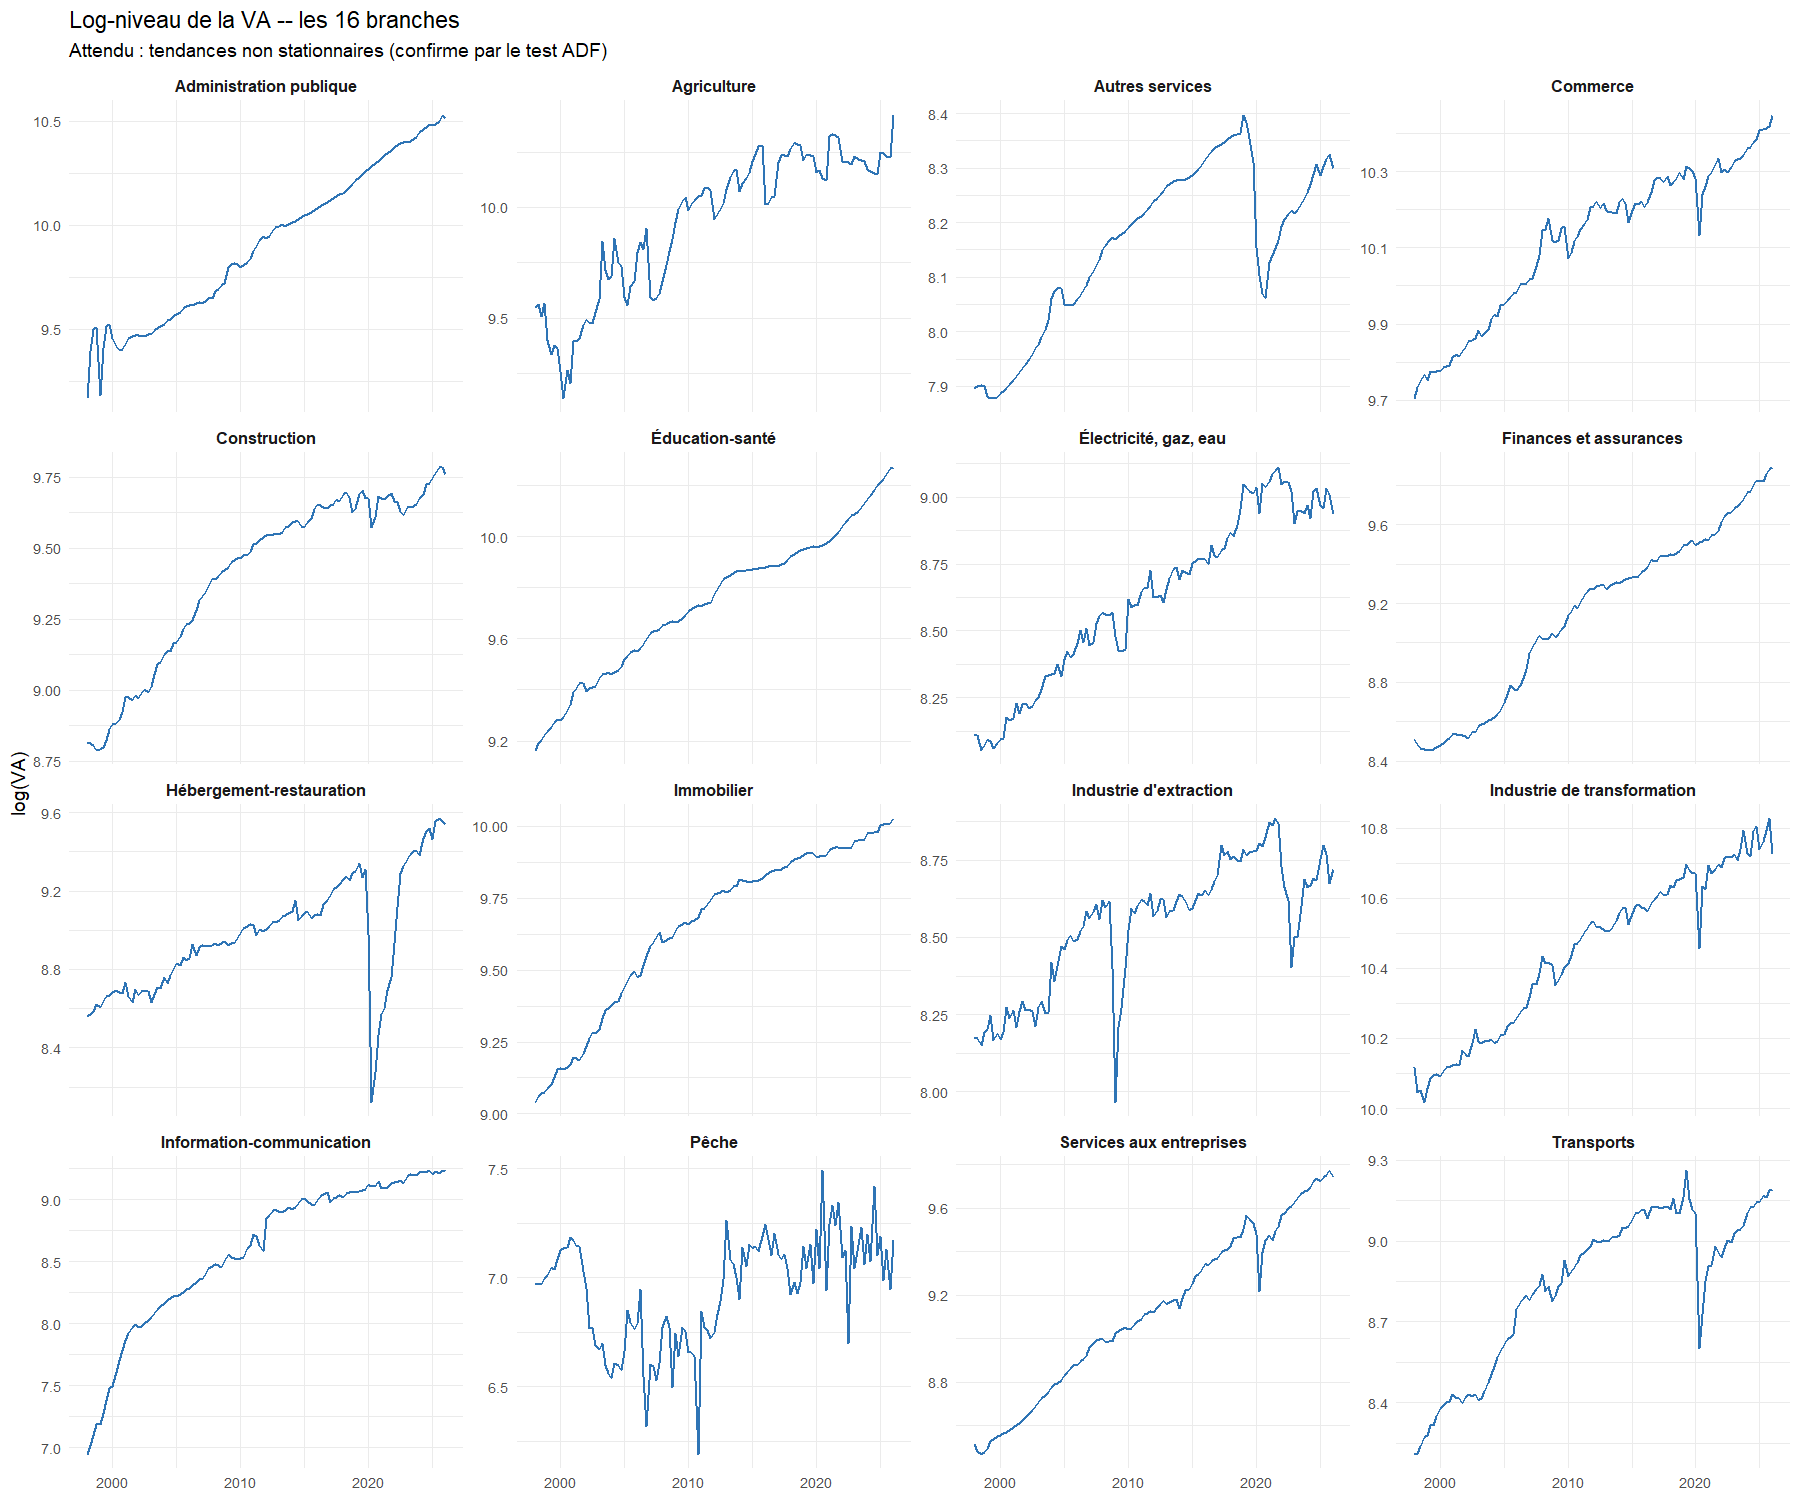
\includegraphics[width=0.95\textwidth]{figures/01a_toutes_branches_log_niveau.png}
\caption{Log-niveau de la valeur ajoutée des 16 branches --- des tendances visibles, non stationnaires, confirmées par le test ADF.}
\end{figure}

\begin{figure}[H]
\centering
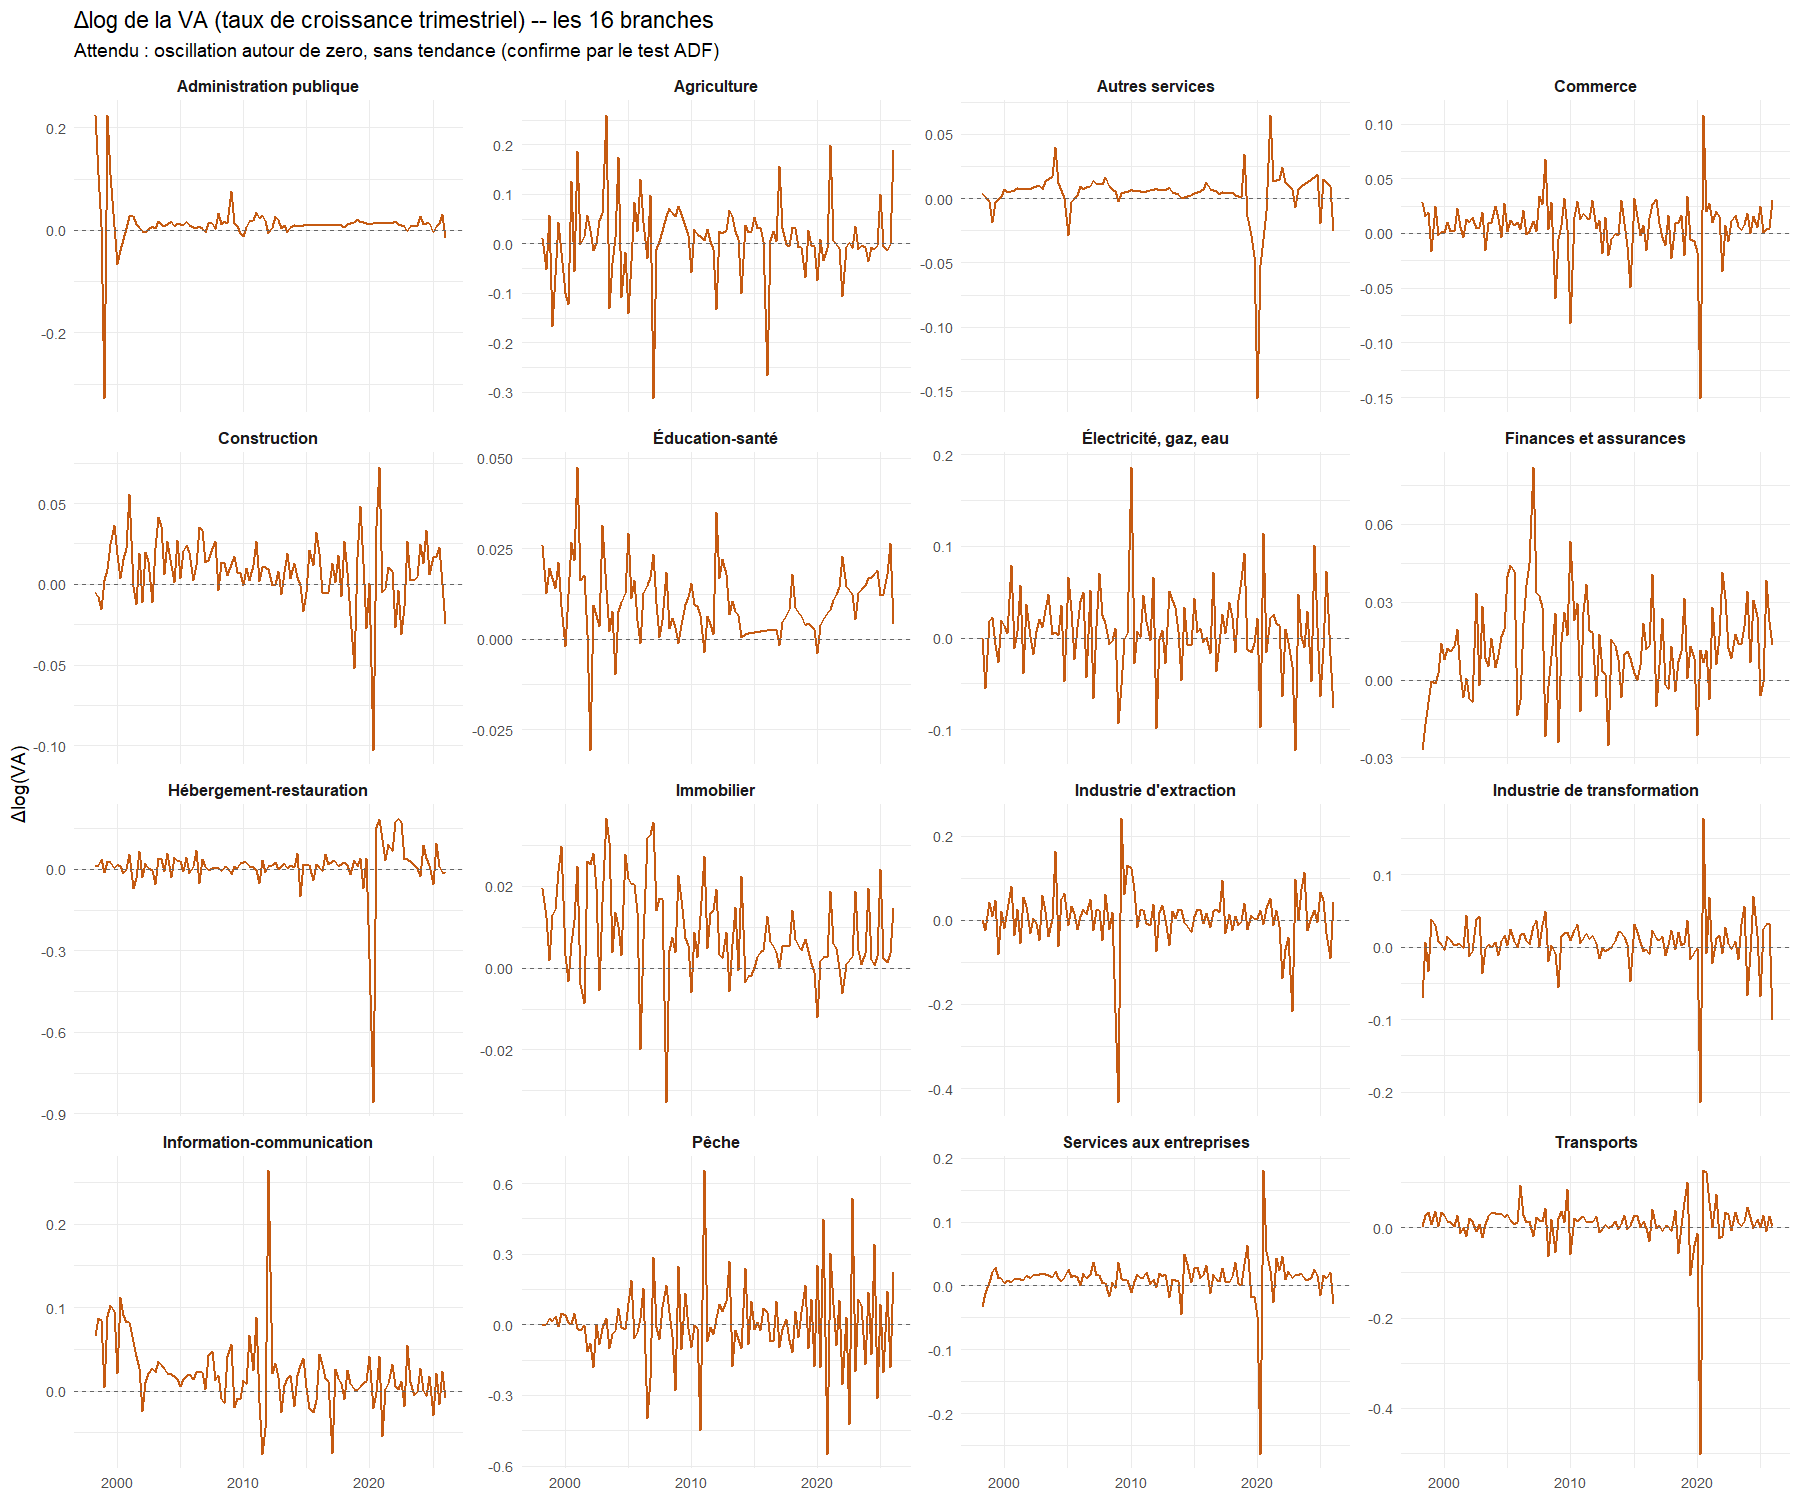
\includegraphics[width=0.95\textwidth]{figures/01b_toutes_branches_deltalog.png}
\caption{Taux de croissance trimestriel ($\Delta\log$) des 16 branches --- oscillation autour de zéro, sans tendance visible, cohérente avec la stationnarité confirmée.}
\end{figure}

% ============================================================================
\section{Le prior Minnesota : l'idée centrale}
% ============================================================================

\subsection{Un prior bayésien, déguisé en données}

\begin{definitionbox}
\textbf{Résultat mathématique central.} Imposer un prior gaussien $\theta \sim \mathcal{N}(\theta_0, \Omega)$ sur les coefficients d'un modèle $y = X\theta + \varepsilon$ est \textbf{mathématiquement équivalent} à ajouter des \emph{observations fictives} $(y^d, X^d)$ telles que $y^d = X^d\theta_0$, puis à estimer un simple OLS sur l'ensemble des données réelles et fictives empilées.
\end{definitionbox}

Pourquoi cette équivalence tient : l'estimateur qui maximise la probabilité a posteriori (MAP) résout
\begin{equation}
\hat\theta_{MAP} = \arg\min_\theta \underbrace{\sum_t (y_t - x_t\theta)^2}_{\text{ajustement aux données}} + \underbrace{\sigma^2(\theta - \theta_0)'\Omega^{-1}(\theta-\theta_0)}_{\text{pénalité de distance au prior}}
\label{eq:map}
\end{equation}
--- une régression pénalisée, structurellement identique à une régression ridge. Ajouter des lignes de données fictives $(y^d=X^d\theta_0)$ et faire un simple OLS sur l'ensemble redonne exactement cette même solution, \textbf{sans jamais avoir à manipuler $\Omega^{-1}$ explicitement} : c'est ce qui rend la méthode de Bańbura, Giannone \& Reichlin$\cit{2}$ si simple à implémenter en pratique.

\subsection{Pourquoi $\delta_i = 0$ pour nos 16 branches}
\label{sec:delta}

Le paramètre $\delta_i$ est le \emph{centre} du prior --- la réponse à la question : \emph{« en l'absence de toute donnée, que devrais-je croire par défaut sur le premier retard de la variable $i$ ? »}

\begin{definitionbox}
\textbf{Les deux régimes possibles.}
\begin{align*}
\delta_i = 1 &\quad\text{(marche aléatoire)} : \quad y_t = y_{t-1} + \varepsilon_t \\
\delta_i = 0 &\quad\text{(retour à la moyenne)} : \quad y_t = 0 + \varepsilon_t
\end{align*}
Higgins$\cit{1}$ utilise $\delta_i=1$ pour ses composantes en log-niveau (une hypothèse adaptée à des niveaux qui évoluent lentement, où « hier » est une bonne approximation d'« aujourd'hui »). Pour une variable stationnaire en $\Delta\log$ --- notre cas, confirmé section précédente --- le comportement naturel est une oscillation autour de zéro, pas une dérive : $\delta_i=0$ est donc le choix statistiquement cohérent.
\end{definitionbox}

\begin{resultatbox}
\textbf{Conclusion} : nos 16 branches utilisent $\delta_i=0$ pour toutes, une décision directement justifiée par le résultat empirique du test ADF (16/16 stationnaires en $\Delta\log$), pas une simple reconduction de la règle de Higgins.
\end{resultatbox}

% ============================================================================
\section{Les trois blocs d'observations fictives}
% ============================================================================

Le prior Minnesota complet répond en réalité à \textbf{trois questions distinctes}, portant sur trois objets mathématiques différents du modèle --- les coefficients $A_l$, la matrice de covariance des résidus $\Sigma$, et la constante $c$. Chacun nécessite son propre bloc d'observations fictives ; les mélanger n'aurait pas de sens mathématique.

\subsection{Bloc 1 --- Prior sur les coefficients $A_l$}

\textbf{Question} : comment chaque branche dépend-elle de son propre passé et de celui des autres ?

Pour chaque retard $l=1,\dots,p$, on ajoute une observation fictive par branche :
\begin{equation}
Y^{d1}_l = 0_{n\times n}, \qquad X^{d1}_l = \text{diag}\left(\frac{\sigma_1\cdot l}{\lambda}, \ \dots, \ \frac{\sigma_{16}\cdot l}{\lambda}\right)
\label{eq:bloc1}
\end{equation}

\begin{intuition}
\textbf{Pourquoi une matrice diagonale} : chaque observation fictive ne contraint que le coefficient d'une branche sur \emph{son propre} retard --- aucune contrainte fictive sur les effets croisés entre branches, qui restent déterminés uniquement par les vraies données.

\textbf{Pourquoi diviser par $\lambda$} : plus $\lambda$ est petit, plus le terme est grand, plus l'observation fictive pèse dans la régression augmentée, plus le coefficient est tiré vers $\delta_i=0$. C'est le curseur central du prior (section \ref{sec:lambda}).

\textbf{Pourquoi multiplier par $l$} : les retards lointains sont contraints plus fortement que les retards récents --- le tableau ci-dessous l'illustre avec $\sigma_i=0{,}02$, $\lambda=0{,}15$ :
\begin{center}
\begin{tabular}{ccc}
\toprule
Retard $l$ & $\sigma_i \cdot l / \lambda$ & Force de la contrainte \\
\midrule
1 & 0{,}133 & la plus faible \\
5 & 0{,}667 & la plus forte \\
\bottomrule
\end{tabular}
\end{center}
Cohérent avec l'intuition que le trimestre dernier renseigne plus sur aujourd'hui que le trimestre d'il y a plus d'un an.

\textbf{Pourquoi diviser par $\sigma_i$} : sans ce terme, une branche très volatile et une branche très stable seraient contraintes de façon identique en valeur absolue --- absurde, puisqu'un coefficient de 0,3 est énorme pour une série stable et négligeable pour une série très bruitée. Diviser par $\sigma_i$ exprime la contrainte \emph{relativement à l'échelle propre de chaque branche} (section \ref{sec:sigma}).
\end{intuition}

\subsection{Bloc 2 --- Prior sur la matrice de covariance des résidus $\Sigma$}

\textbf{Question} : la matrice de covariance des 16 résidus est-elle numériquement bien posée ?

\begin{equation}
Y^{d2} = \text{diag}(\sigma_1,\dots,\sigma_{16}), \qquad X^{d2} = 0
\end{equation}

Avec 16 équations, $\Sigma$ compte $16\times17/2=136$ éléments distincts à estimer --- sans cette contrainte minimale, elle peut devenir singulière ou mal conditionnée, ce qui ferait échouer l'inversion $(X_{\text{aug}}^\top X_{\text{aug}})^{-1}$ nécessaire à l'estimation.

\subsection{Bloc 3 --- Prior (quasi neutre) sur la constante}

\textbf{Question} : quel est le niveau moyen de croissance de chaque branche ?

\begin{equation}
X^{d3}_{1,1} = \epsilon = 10^{-5}
\end{equation}

Aucune contrainte économique ne doit peser sur la constante --- elle doit refléter purement le niveau moyen observé dans les données. Le $\epsilon$ minuscule rend cette ligne fictive quasiment neutre, tout en la rendant formellement nécessaire à la construction de la matrice.

\begin{resultatbox}
\textbf{Synthèse.} Ce ne sont pas trois répétitions prudentes du même mécanisme : ce sont \textbf{trois paramètres mathématiquement distincts} ($A_l$, $\Sigma$, $c$), chacun nécessitant sa propre régularisation. Retirer un bloc laisserait cette dimension précise du modèle totalement libre, sans protection contre le sur-ajustement sur cette partie.
\end{resultatbox}

% ============================================================================
\section{Le calcul de $\sigma_i$ : l'échelle propre de chaque branche}
\label{sec:sigma}
% ============================================================================

\subsection{Pourquoi la variance résiduelle, pas la variance brute}

\begin{definitionbox}
$\sigma_i$ n'est \textbf{pas} l'écart-type brut de la série $i$ --- c'est l'écart-type des \textbf{résidus} d'un AR($p$) univarié ajusté sur le $\Delta\log$ de la branche $i$, prise isolément :
\begin{equation}
y_{i,t} = \phi_1 y_{i,t-1} + \dots + \phi_p y_{i,t-p} + u_{i,t}, \qquad \sigma_i = \sqrt{\widehat{\text{Var}}(u_{i,t})}
\end{equation}
\end{definitionbox}

\begin{intuition}
Si on utilisait l'écart-type brut, une branche à forte autocorrélation (des cycles longs et réguliers) paraîtrait « volatile » alors qu'une bonne partie de cette variation est en réalité \emph{prévisible} depuis son propre passé --- donc pas du vrai bruit. La variance résiduelle isole la part réellement imprévisible, celle qui doit calibrer la force du prior.
\end{intuition}

\subsection{Résultat empirique}

\begin{resultatbox}
\begin{center}
\small
\begin{tabular}{lcc}
\toprule
\textbf{Branche} & $\sigma_i$ & Écart-type brut \\
\midrule
Pêche (la plus volatile) & 0{,}14792 & 0{,}17506 \\
Hébergement-restauration & 0{,}09817 & 0{,}10049 \\
Industrie de transformation & 0{,}03297 & 0{,}03682 \\
Finances et assurances & 0{,}01658 & 0{,}01774 \\
Éducation-santé (la plus stable) & 0{,}00741 & 0{,}00962 \\
\bottomrule
\end{tabular}
\end{center}
\end{resultatbox}

L'écart entre la branche la plus volatile (Pêche) et la plus stable (Éducation-santé) est d'un facteur \textbf{20} --- cohérent avec l'intuition économique : la pêche dépend d'aléas naturels et saisonniers forts, tandis que les services publics d'éducation-santé évoluent de façon très régulière.

\begin{figure}[H]
\centering
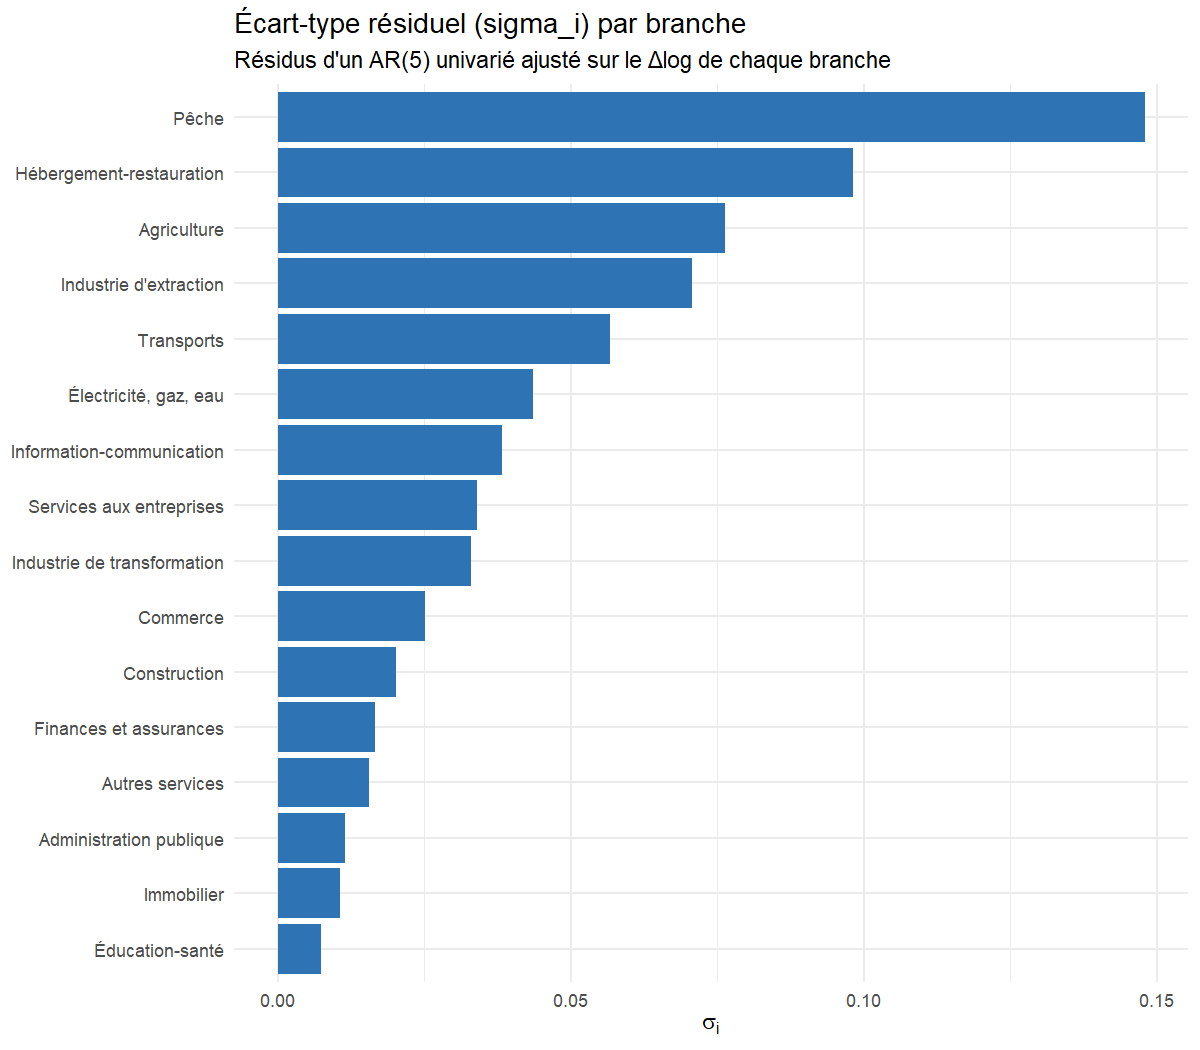
\includegraphics[width=0.75\textwidth]{figures/02_sigma_i_par_branche.png}
\caption{Écart-type résiduel $\sigma_i$ par branche, classé du plus volatile au plus stable.}
\end{figure}

% ============================================================================
\section{Le choix de $\lambda$ : l'intensité du rétrécissement}
\label{sec:lambda}
% ============================================================================

\subsection{Ce que $\lambda$ contrôle}

Reprenons la formule du bloc 1 (équation \ref{eq:bloc1}). Aux deux extrêmes :

\begin{align*}
\lambda \to \infty &: \quad \frac{\sigma_i l}{\lambda} \to 0 \quad\Rightarrow\quad \text{observation fictive neutre} \quad\Rightarrow\quad \text{OLS classique, sur-ajustement possible} \\
\lambda \to 0 &: \quad \frac{\sigma_i l}{\lambda} \to \infty \quad\Rightarrow\quad \text{le modèle est forcé vers } \delta_i=0, \text{ ignore les données}
\end{align*}

$\lambda$ est un curseur continu entre ces deux extrêmes --- le bon $\lambda$ minimise la vraie erreur de prévision, ni trop de biais, ni trop de variance.

\subsection{La méthode de calibration retenue}

\begin{definitionbox}
\textbf{Principe retenu} : $\lambda$ est choisi pour minimiser le RMSFE (Root Mean Square Forecast Error) \textbf{hors échantillon}, par évaluation en fenêtre glissante sur une période de validation (les 23 derniers trimestres, 2020T3--2026T1), jamais en ajustement en échantillon.

Chaque valeur de $\lambda$ testée implique de \textbf{ré-estimer entièrement le BVAR à chaque origine glissante}, avec seulement les données disponibles jusqu'à cette origine --- aucune fuite d'information vers le futur.
\end{definitionbox}

Cette méthode s'inspire directement de celle utilisée par Higgins$\cit{1}$ lui-même pour calibrer son propre BVAR mixte-fréquence : \emph{« $\lambda=0{,}10$ a été retenu car il donnait la meilleure performance de prévision parmi les valeurs 0,05, 0,10, 0,15, 0,20 et 0,25 »} (annexe, implémentation des BVAR).

\subsection{Résultat empirique}

\begin{resultatbox}
\begin{center}
\begin{tabular}{cc}
\toprule
$\lambda$ & RMSFE (hors échantillon) \\
\midrule
0{,}01 & 0{,}080017 \\
0{,}02 & 0{,}079663 \\
0{,}03 & 0{,}079339 \\
\textbf{0{,}05} & \textbf{0{,}079321} \\
0{,}10 & 0{,}081776 \\
0{,}15 & 0{,}084607 \\
0{,}20 & 0{,}087400 \\
0{,}30 & 0{,}093413 \\
\bottomrule
\end{tabular}
\end{center}
\end{resultatbox}

\begin{figure}[H]
\centering
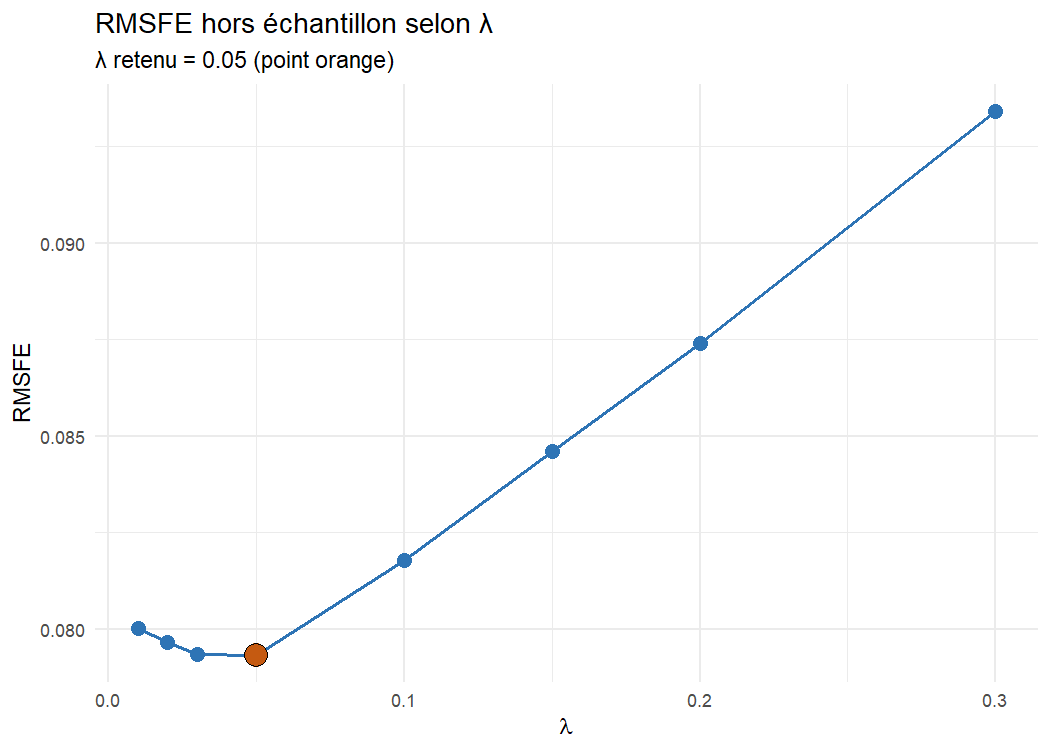
\includegraphics[width=0.6\textwidth]{figures/03_rmsfe_par_lambda.png}
\caption{RMSFE hors échantillon selon $\lambda$ --- un minimum intérieur, pas un minimum de bord de grille.}
\end{figure}

\textbf{Lecture du résultat} : le RMSFE décroît de $\lambda=0{,}01$ à $\lambda\approx0{,}05$, puis remonte nettement au-delà --- un \textbf{vrai minimum intérieur}, confirmant que la grille testée couvre bien la zone d'intérêt (contrairement à un minimum qui serait resté au bord de la grille, signe qu'il faudrait tester encore plus loin).

\begin{intuition}
\textbf{Réserve statistique honnête} : l'écart entre $\lambda=0{,}03$ (0,079339) et $\lambda=0{,}05$ (0,079321) est minuscule --- ces deux valeurs sont statistiquement quasi indiscernables sur seulement 23 trimestres de validation. Le bon message n'est pas « $\lambda=0{,}05$ est le meilleur », mais « la zone $\lambda\in[0{,}03\,;\,0{,}05]$ est clairement préférable à $\lambda\geq0{,}10$ ».
\end{intuition}

% ============================================================================
\section{Estimation finale et vérification de stabilité}
% ============================================================================

\subsection{L'estimation par OLS augmenté}

Une fois les trois blocs construits, les observations réelles et fictives sont empilées :
\begin{equation}
Y_{\text{aug}} = \begin{pmatrix} Y_{\text{réel}} \\ Y^{d1} \\ Y^{d2} \\ Y^{d3}\end{pmatrix}, \qquad
X_{\text{aug}} = \begin{pmatrix} X_{\text{réel}} \\ X^{d1} \\ X^{d2} \\ X^{d3}\end{pmatrix}, \qquad
\hat B = (X_{\text{aug}}^\top X_{\text{aug}})^{-1} X_{\text{aug}}^\top Y_{\text{aug}}
\end{equation}

Un simple OLS sur des données augmentées --- c'est ce qui rend la méthode de Bańbura, Giannone \& Reichlin$\cit{2}$ si élégante : aucun solveur bayésien complexe n'est nécessaire.

\subsection{Pourquoi vérifier la stabilité}

\begin{definitionbox}
Un VAR($p$) s'écrit sous forme compagne comme un VAR(1) sur un vecteur étendu de dimension $n\times p$. Le VAR est \textbf{stable} (stationnaire) si et seulement si toutes les valeurs propres de la matrice compagne $F$ ont un module strictement inférieur à 1 :
\[
\max_k |\text{valeur propre}_k(F)| < 1
\]
\end{definitionbox}

\begin{intuition}
Un VAR instable produirait des prévisions qui \emph{divergent} dans le temps (une croissance qui s'auto-amplifie indéfiniment) --- un défaut qu'aucun indicateur de performance à un seul pas (RMSFE, test de Diebold-Mariano) ne détecte directement. Ce test est la garantie que le modèle est mathématiquement bien posé pour la prévision, indépendamment de sa précision.
\end{intuition}

\subsection{Résultat}

\begin{resultatbox}
\textbf{Module maximal observé : 0,4442} --- largement inférieur à 1. \textbf{Le VAR est stable.} Cohérent avec un $\lambda$ faible (0,05) : un prior fortement contraignant pousse naturellement les coefficients vers un système peu persistant, donc stable.
\end{resultatbox}

\begin{figure}[H]
\centering
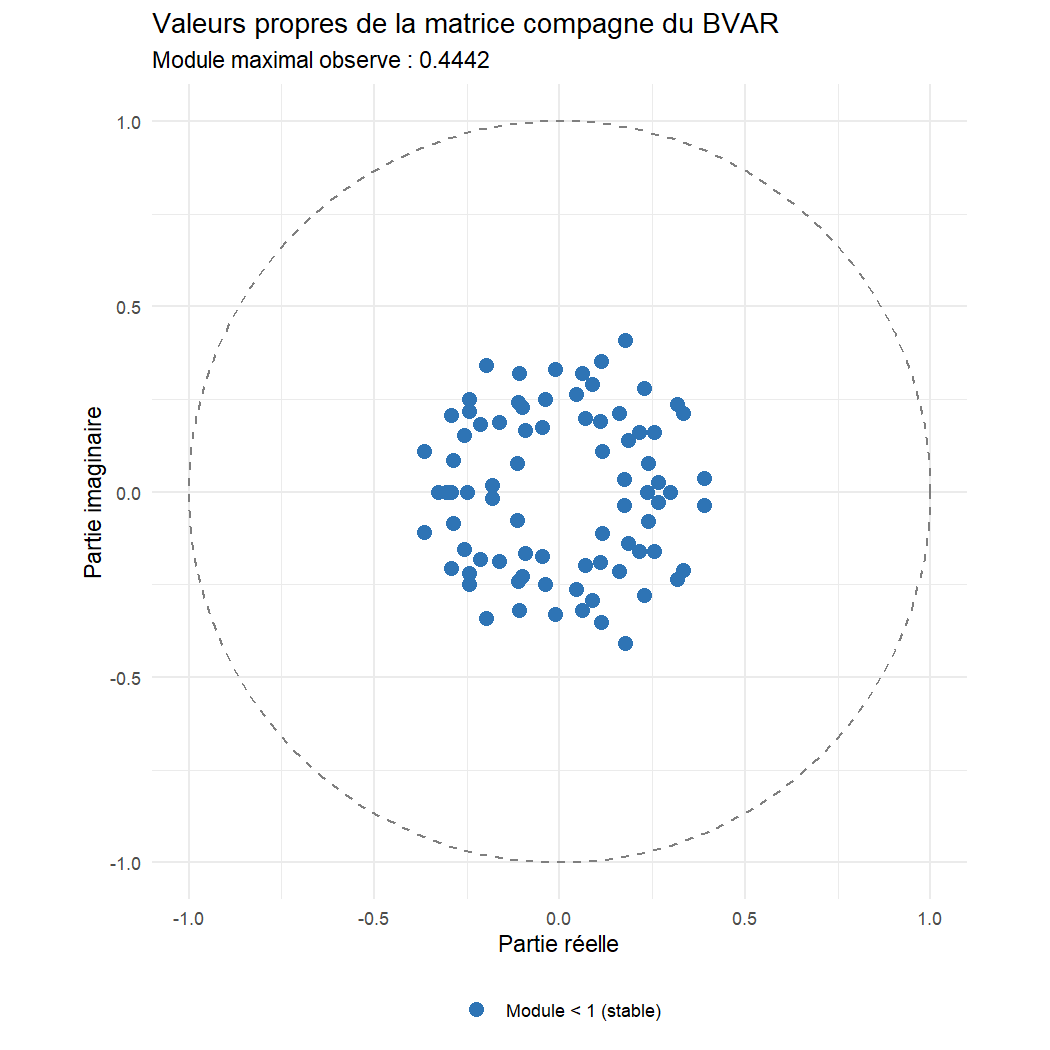
\includegraphics[width=0.55\textwidth]{figures/04_cercle_unite_valeurs_propres.png}
\caption{Valeurs propres de la matrice compagne dans le plan complexe --- toutes à l'intérieur du cercle unité.}
\end{figure}

% ============================================================================
\section{Conclusion de la Phase 1}
% ============================================================================

Le tableau suivant résume l'ensemble des choix méthodologiques de cette phase, chacun rattaché à sa justification :

\begin{resultatbox}
\begin{center}
\small
\begin{tabular}{p{3.2cm}p{3cm}p{7.5cm}}
\toprule
\textbf{Choix} & \textbf{Valeur retenue} & \textbf{Justification} \\
\midrule
Transformation & $\Delta\log$ & Test ADF : 16/16 branches stationnaires (contre 1/16 en niveau) \\
$\delta_i$ & 0 pour toutes & Cohérent avec la stationnarité en $\Delta\log$ (retour à la moyenne) \\
$p$ (retards) & 5 & Cohérence avec Higgins$\cit{1}$ (non re-testé) \\
$\sigma_i$ & Calculé par branche & Écart-type résiduel d'un AR(5) univarié, pas l'écart-type brut \\
$\lambda$ & 0,05 (zone 0,03--0,05) & Minimum du RMSFE hors échantillon, sur grille inspirée de Higgins$\cit{1}$ \\
Stabilité & Confirmée (module max 0,4442) & Toutes les valeurs propres de la matrice compagne $<1$ \\
\bottomrule
\end{tabular}
\end{center}
\end{resultatbox}

Le BVAR trimestriel constitue la première brique du modèle complet de nowcasting --- il fournit une prévision de repli pour les 16 branches, y compris celles ne disposant d'aucun indicateur mensuel validé, et sera combiné aux équations de passerelle (\emph{bridge equations}) dans la phase suivante.

% ============================================================================
\section*{Références}
\addcontentsline{toc}{section}{Références}
% ============================================================================
\begin{enumerate}[leftmargin=1.6em, label=\textbf{[\arabic*]}]
\item \hypertarget{ref1}{} Higgins, P. (2014). \textit{GDPNow: A Model for GDP ``Nowcasting''}. Federal Reserve Bank of Atlanta, Working Paper 2014-7.
\item \hypertarget{ref2}{} Bańbura, M., Giannone, D. \& Reichlin, L. (2010). \textit{Large Bayesian Vector Auto Regressions}. Journal of Applied Econometrics, 25(1), 71--92.
\item \hypertarget{ref3}{} Litterman, R. (1986). \textit{Forecasting with Bayesian Vector Autoregressions --- Five Years of Experience}. Journal of Business \& Economic Statistics, 4(1), 25--38.
\item \hypertarget{ref4}{} Dickey, D.A. \& Fuller, W.A. (1979). \textit{Distribution of the Estimators for Autoregressive Time Series with a Unit Root}. Journal of the American Statistical Association, 74(366), 427--431 ; version augmentée : Said, S.E. \& Dickey, D.A. (1984), Biometrika, 71(3), 599--607.
\end{enumerate}

\end{document}
